\documentclass[a4paper, 12pt, twoside]{article}
\usepackage[T2A,T1]{fontenc}
\usepackage[utf8]{inputenc}
\usepackage[english, russian]{babel}
\usepackage{graphicx}
\usepackage[hcentering, bindingoffset = 10mm, right = 15 mm, left = 15 mm, top=20mm, bottom = 20 mm]{geometry}
\usepackage{multirow}
\usepackage{ctable}
\usepackage{lipsum}
\usepackage{amsmath, amstext}
\usepackage{siunitx}
\usepackage{subcaption}
\usepackage{wrapfig}
\usepackage{adjustbox}
\usepackage{enumerate, indentfirst, float}
\usepackage{capt-of, svg}
\usepackage{cmap} % Улучшенный поиск русских слов в полученном pdf-файле

\usepackage{pscyr} % Нормальные шрифты
\usepackage[normalem]{ulem} % для подчёркиваний uline
\ULdepth = 0.16em
%% Перенос знаков в формулах (по Львовскому)
\newcommand*{\hm}[1]{#1\nobreak\discretionary{}
	{\hbox{$\mathsurround=0pt #1$}}{}}

\usepackage{fancyhdr} %Колонтикулы
\pagestyle{fancy}
\lhead{
\includegraphics[width = 10 mm]{logo.jpg} Связанные колебательные контуры.}
\rhead{\textit{\today}}

\newenvironment{bottompar}{\par\vspace*{\fill}}{\clearpage}
 
\begin{document}
\begin{titlepage}

\newcommand{\HRule}{\rule{\linewidth}{0.7mm}} % Defines a new command for the horizontal lines, change thickness here

\center % Center everything on the page
 
%----------------------------------------------------------------------------------------
%	HEADING SECTIONS
%----------------------------------------------------------------------------------------

\textsc{\LARGE Московский Физико-Технический Институт}\\[1,5cm] % Name of your university/college

\textsc{\large Лабораторная работа по радиотехническим сигналам и цепям}\\[0.5cm] % Minor heading such as course title

%----------------------------------------------------------------------------------------
%	TITLE SECTION
%----------------------------------------------------------------------------------------

\HRule
\\[0.4cm]
{ \huge \bfseries Связанные колебательные контуры.}
\\[0.4cm] % Title of your document
\HRule
\\[1.5cm]


 
%----------------------------------------------------------------------------------------
%	AUTHOR SECTION
%----------------------------------------------------------------------------------------


	\begin{center} \large
		\textbf{Автор:}\\
		Глеб Уваркин \\
		615 группа
	\end{center}

~


\begin{bottompar}
	\begin{center}
		
\includegraphics[width = 80 mm]{logo.jpg}
	\end{center}
	{\large \today}

\end{bottompar}
\vfill % Fill the rest of the page with whitespace

\end{titlepage}
\begin{figure}[H]
	\centering
	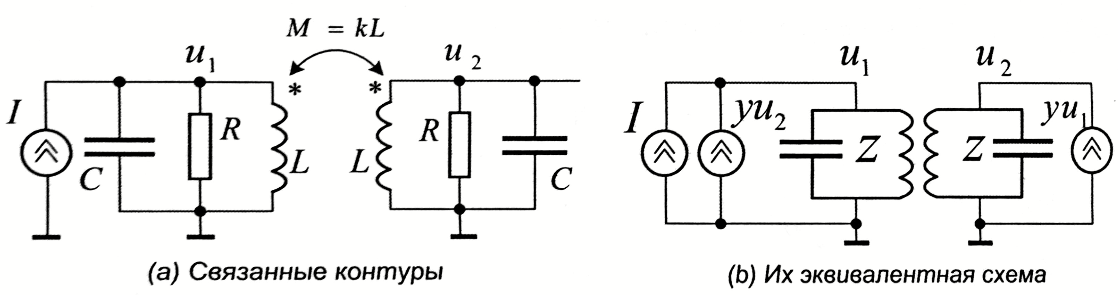
\includegraphics[width =  0.9\linewidth]{cvk}
	\caption{Связанные контуры.}
\end{figure}

\section*{Задание №1. Система с индуктивной связью.}

\textbf{3.} Изучим поведение резонансных кривых и фазовых характеристик при $F = [0.2, 1|0.2]$ и $F = [1.5|1]$. Измерим границы диапазонов изменения фаз на первом и втором контурах: 

на первом контуре -- от $-84.161^{\circ}$ до $84.415^{\circ}$, на втором контуре -- от $-258.322^{\circ}$ до $78.322^{\circ}$,

а также разность фаз между напряжениями на контурах на частоте $f_0$: $89.238^{\circ}$.

Измерив уровни $u_1(f_0)$, $u_2(f_0)$ при $F = 0.5;~1;~2$, проверим формулы 
\begin{equation}
\label{f1}
u_1(f_0) = \frac{1}{1+F^2},~u_2(f_0)= \frac{F}{1+F^2}
\end{equation}

\begin{table}[H]
	\centering
	\caption{Проверка формулы \eqref{f1}.}
	\begin{tabular}{c|ccc} \toprule
		$F$                         & $1$ & $0.5$ & $2$ \\ \midrule
		$u_1(f_0)_{Mccap}$          & 0.5 & 0.8   & 0.2 \\
		$u_1(f_0)_{\text{формула}}$ & 0.5 & 0.8   & 0.2 \\
		$u_2(f_0)_{Mccap}$          & 0.5 & 0.4   & 0.2 \\
		$u_2(f_0)_{\text{формула}}$ & 0.5 & 0.4   & 0.2 \\ \bottomrule
	\end{tabular}
\end{table}

$\Longrightarrow$ формула \eqref{f1} выполняется.

~

\textbf{4.} Измерим значения $F$, при которых возникает: a) провал на первом контуре: $F = 0.6$, b) провал на втором контуре: $F = 1.1$, c) подъём на фазовой характеристике первого контура: $F = 1.1$.

Измерив частоты пересечения нуля фазовой характеристикой $u_1$ при $F = 5$ ($\nu \hm{=} 976.121k,~1.001M,~1.025M$) и при $F = 10$ ( $\nu = 953.430k,~1.005M,~1.054M$), проверим приближённые ($f_0\pm FF_0$) и уточнённые ($f_0\sqrt{1\pm\frac{F}{Q}}$).

~

\textbf{5.} Оставим только плот 1. При критической связи измерим ширину полосы по уровню -3dB эталонного контура ($\Delta f = 10.273k$) и ширину полосы по уровню -9dB резонансной кривой на втором контуре ($\Delta f = 14.279k$). Убедимся, что их отношение составляет $\sqrt{2}$.

Измерим уровни затухания критической кривой при сдвигах по частоте на декаду $F_0$, то есть на $\pm 10F_0 = \pm 50k$ (затухание -- $-34\frac{dB}{\text{дек}_{F_0}}$). Варьируя сопротивление потерь эталонного контура $R = [60k,~80k|5k]$, выясним, что при добротности $Q = 68.6$ ($R \hm{=} 70k,~\Delta f = 14.557k$) его полоса сравнивается с полосой двухконтурной системы. Измерим затухание, вносимое эталонным контуром с этой добротностью при расстройках на декаду $F_0$ (затухание -- $-16.7\frac{dB}{\text{дека}_{F_0}}$). Оценим выигрыш двухконтурной системы по затуханию: выигрыш $\simeq~\text{2 раза}$.

~

\textbf{6.} Изучим поведение резонансных кривых при $F \hm{=} [0.5,~1|0.1]$. Найдём значение $F \hm{=} [0.65,~0.75|0.05]$, при котором полоса двухконтурной системы по критическому уровню -9dB сравнивается с полосой $10k$ эталонного контура: $F = 0.75$. При этом значении $F$ оценим выигрыш по затуханию при расстройке на декаду $F_0$ двухконтурной системы по сравнению с эталоном: у эталона -- $-19.75\frac{dB}{\text{дек}_{F_0}}$, у двухконтурной системы -- $-36.45\frac{dB}{\text{дек}_{F_0}} \Longrightarrow \text{выигрыш $\simeq$ 2 раза}$.

~

\textbf{7.} Измерим значение $F$ из диапазона $F = [2.2,~2.6|0.1]$, при котором полоса двухконтурной системы по критическому уровню -9dB сравнивается с полосой $10k$ эталонного контура.($F = 0.75$). При этом значении $F$ измерим ширину полосы $\Delta \omega$ двухконтурной системы по уровню -9dB ($\Delta \omega = 30.532k$) и уровни затухания при расстройках на декаду $F_0$ (у эталона -- $-23\frac{db}{\text{дек}}$, у двухконтурной системы -- $-19.833\frac{dB}{\text{дек}}$). Варьированием сопротивления эталонного контура $R$ добьёмся совпадения его полосы с полосой двухконтурной системы и измерим уровни затухания, вносимого контуром($-18.278\frac{dB}{\text{дек}}$).

~

\textbf{8.} При критической связи $F = 1$ измерим затухания на втором контуре при расстройках на декаду $f_0$. Изучим зависимость уровней затухания от $F = [1,5.5|1.5]$. Занесём результаты в таблицу \ref{t2}.

\begin{table}[H]
	\centering
	\caption{Зависимость уровней затухания от $F$}.
	\label{t2}
	\begin{tabular}{c|cc} \toprule
		& \multicolumn{2}{c}{\begin{tabular}[c]{@{}c@{}}Уровень затухания,\\ $\frac{dB}{\text{дек}}$\end{tabular}} \\ \midrule
		$F$   & \multicolumn{1}{c|}{f = $100k$}                              & f = $10Meg$                              \\ \midrule
		$1$   & \multicolumn{1}{c|}{$-94$}                                   & $-133$                                   \\
		$2.5$ & \multicolumn{1}{c|}{$-85$}                                   & $-126$                                   \\
		$4$   & \multicolumn{1}{c|}{$-82$}                                   & $-122$                                   \\
		$5.5$ & \multicolumn{1}{c|}{$-79$}                                   & $-119$                    \\ \bottomrule              
	\end{tabular}
\end{table} 

~

\textbf{11.} Установив диапазон моделирования $[2Meg, 600k]$, исследуем частотные и фазовые характеристики при сильной связи. Измерим частоты $f_{\pm}$ пиков при $F = 50$: $f_{+} = 1.414M$, $f_{-} = 816.378k$.

\newpage

\section*{Задание №2. Система с ёмкостной связью.}
\textbf{1.} Измерим диапазоны изменения фазовых характеристик на первом и втором контурах:

на 1 контуре -- от $90^{\circ}$ до $-90^{\circ}$

на 2 контуре -- от $-90^{\circ}$ до $-450^{\circ}$.

Измерим значения $F$, при которых возникает: a) провал на первом контуре ($F = 0.5$), b) провал на втором контуре ($F = 1$) c) подъём на фазовой характеристике первого контура ($F = 1$).

Снимем зависимость частоты провала на втором контуре от $F = [2, 4|1]$ (таблица \ref{t3}).

\begin{table}[H]
	\centering
	\caption{Зависимость частоты провала от $F$. }
	\label{t3}
	\begin{tabular}{c|ccc} \toprule
		$F$               & $2$    & $3$    & $4$    \\ \midrule
		$f_{\text{пров}},~\text{Гц}$ & $990k$ & $985k$ & $980k$ \\ \bottomrule
	\end{tabular}
\end{table}

~

\textbf{2.} Измерим уровни затухания при расстройках на $\pm 50k$:

1 контур -- $-17 \frac{dB}{\text{дек}}$

2 контур -- $-35 \frac{dB}{\text{дек}}$.

Перейдём на частотный диапазон $[10Meg,100k]$ и измерим уровни затухания при расстройках на декаду $f_0$:

1 контур -- $-56\frac{dB}{\text{дек}}$

2 контур -- $-94\frac{dB}{\text{дек}}(\text{вблизи $100k$})$, $-133\frac{dB}{\text{дек}}(\text{вблизи $10Meg$})$
\end{document}